\section{Firmware Modul der IMU}
Wie schon zuvor in dem Kapitel erwähnt nutzt das Firmware Modul stark die Driver
und Motion Libarys von STMicroelectronics. Die Software kann in mehrere Teile
geteilt werden, die nacheinander ausgeführt werden. Beim Start werden die
LSM6DSV16X und der LIS2MDL \textbf{initialisiert}, danach werden bei genügend
Daten die \textbf{Sensoren ausgelesen}, \textbf{Sensor Kalibration} durchgeführt, die
Kalibrierten Daten an den \textbf{Sensor Fusion Algorithmus} weitergegeben. In
den Abbildungen \ref{X} wird die physicher Verbindung von MCU, IMU
und Magnetometer gezeigt. Abbildung \ref{Y} zeigt den Abstrakten Programmablauf
beim IMU auslesen
\begin{figure}[h]
    \centering
    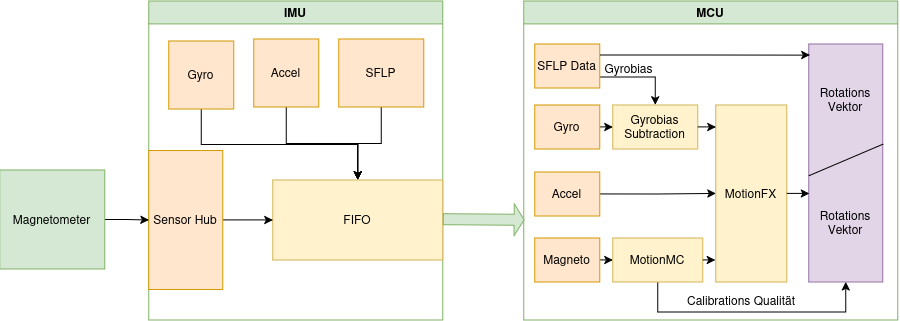
\includegraphics[width=\textwidth]{Bilder-Grafiken/Matthias/IMU/Datenfluss_IMU_FIRMW.png}
    \caption{Datenfluss zwischen Sensoren und MCU}
\end{figure}

\subsection{Sensor Setup und Configuration}
Bei der Startup der MCU wird jeweils das whoAmI Register der LSM6DSV16X und
LIS2MDL kontrolliert. Damit wird versichert das die Sensoren Antworten und das
der Richtige Sensor eingebaut ist. Danach erfolgt ein Software Reset. Dadurch
wird die IMU in ihre Ausgangskonfiguration zurückgesetzt. Erst danach kann der
Sensor konfiguriert werden.

\subsubsection{LSM6DSV16X}
In der LSM6DSV16X \cite{st_lsm6dsv16x} werden Gyroskop und Accelerometer in den \textit{High
Performance} Moduls gesetzt. Diese laufen mit einer Sample Rate von 240Hz.
\begin{itemize}
    \item \textbf{\textit{Sensor Fusion Low Power} (SFLP)} 
        \cite[Sec. 2.8]{st_lsm6dsv16x} wird dafür genutzt direkt auf dem Sensor 
        6 Achsen Sensor Fusion durch zu führen, den Gravitationsvektor zu
        berechnen und Gyroskop Bias zu bestimmen. 
    \item In den interne \textbf{FIFO} \cite[Sec. 6.12]{st_lsm6dsv16x} wird so
        konfiguriert, dass alle Sensor Daten in ihm zwischen gespeichert werden
        und dann mehrere Batches nacheinander auszulesen. Es wird Gyroskop,
        Accelerometer, Daten vom Sensor-Hub (Magnetometer) und alle Daten vom
        SFLP-Block darin gespeichert. Noch dazu wird pro Sensor Batch ein
        Zeitstempel gespeichert. In Kapitel \ref{fifo_batch} wird die Batch
        Funktion und der Ausleseintervall weiter erklärt.
\end{itemize}

\subsubsection{LIS2MDL}
Das Magnetometer muss im Vergleich zur IMU wenig konfiguriert werden. Bei der
Konfiguration wird es auf High Performance Mode gesetzt, wie auch die
automatische Temperatur Compensation eingeschalten.
Danach wird der Sensor-Hub der LSM6DSV16X dafür konfiguriert, die X-,Y-,Z-Achsen
ausgelesen werden.\\
Der Sensor-Hub ließt neue Werte mit 30Hz aus. Da die LIS2MDL selbst nicht keine
30Hz Sample Rate unterstützt (nur 20Hz oder 50Hz), over sampled sie mit 50Hz.
Damit wird verhindert, dass die MCU doppelte/veraltete Daten bekommt.

\subsection{IMU auslesne}
Das auslesen wird über den Interrupt Pin der IMU ausgelöst, diese findet statt
wenn der FIFO mindestens 30 Batches enthält. Bei diesem Ereignis wird der FIFO
von der MCU entleert. 
\subsubsection{FIFO und Batches\cite[Sec. 6.12]{st_lsm6dsv16x}} \label{fifo_batch}
Der FIFO ist in Batches und weiter in 7Byte große Einträge unterteilt. Ein
Eintrag besteht jeweils aus einem Tag-Byte und 6 Byte an Daten. Mit dem Tag kann
man bestimmen, zu welchem Batch der Eintrag gehört und welche Art von Daten es
sind (Gyroskop, Accelerometer, ...). In Abbildung \ref{fig:fifo_aufbau} ist der
Aufbau des FIFOs visualisiert. 

\begin{figure}[h]
    \centering
    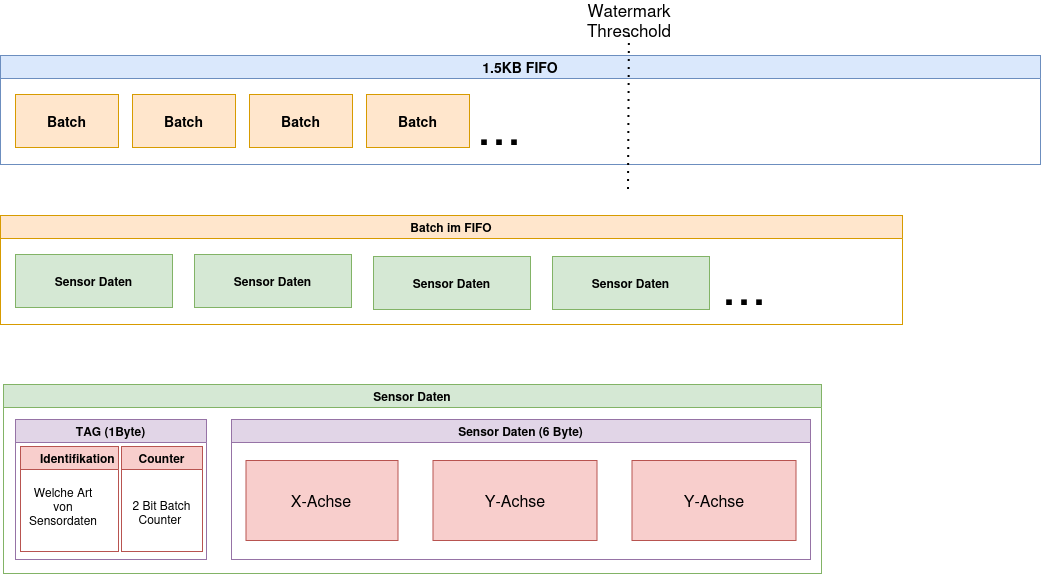
\includegraphics[width=\textwidth]{Bilder-Grafiken/Matthias/IMU/Fifo_Visualisierung.png}
    \caption{Visualisierung des FIFOs der LSM6DSV16X}
    \label{fig:fifo_aufbau}
\end{figure}

%% --- der teil wurde rausgenommen, weil der inhalt sonst zu viel 
%%               und kompliziert geworde wär ---
%Noch dazu wird der IMU eingestellt, dass sie
%nach 30 gespeicherten Baches im FIFO einen Interrupt auslösen soll.
%Dadurch wird die MCU nicht mit Interrupts von 240Hz Intervall
%überflutet und können trotzdem mit einer hohen Sample Rate messen. Der
%Nachteil dabei ist das es eine höhere Latenz gibt bis die MCU auf eine
%Orientierungsänderung Reagieren kann.

\subsection{Sensor calibration} 
\subsubsection{Gyroskop Bias}
Der Gyro Bias Berechnung wird von dem SFLP-Block gemacht. Diese muss von der MCU
nur noch von dem Messwert Subtrahiert werden. 

\subsubsection{Magnetometer cal}
Für die Hardiron- und Softireon-Offset Kalibration für das Magnetometer wurde
die MotionMC Library von STMicroelectronics \cite{st_motionMC} benutzt. Dieser
werden die Sensordaten in $\mu\text{T}$ übergeben. Diese Verarbeitet die Daten 
weiter und gibt kalibrierte Daten, wie auch die Qualität der Calibration aus.

%% --- zeitstemple calibreirung rausgelaassen weil es zu nischig ist ---
%\subsubsection{ocilator calibration register}
%Die LSM6DSV16X hat einen internen Oscillator (46.08Hz; anahme von formel,
%datenblatt gibt nur typ 21.75us an, formel für freq fine reg lässt glauben das
%es nominal 46,08 ist,), auf dem alles basieret, um exakte timestamps/sampele
%rates für sensor fusion zu bekommen wird mit freq fine register formel
%convertiert
%kann über das INTERNAL\_FREQ\_FINE register ausgelesen werden, muss auf jeden
%timestamp/odr angewändet weden

\subsection{sensor Fusion}
Für die Verarbeitung der Gyroskop, Accelerometer und Magnetometer werde wurde
die MotionFX Library von STMicroelectronics \cite{st_motionFX} genugzt. Sie
supported 6 Achsen, wie auch 9 Achsen Sensor Fuison. Da die IMU mit dem
SFLP-Block schon eine gute 6 Achsen Fuison bietet, wird die MotionFX parralel
dazu für die 9 Achsen Fusion genutzt. Welche der zwei Orientationen genutzt
wird, hängt davon ab, wie gut die Magnetometer Calibration ist. Fall dieses noch
nicht calibriert ist, oder wieder auf eine schlechte calibration zurückfellt
(Störung durch Umgebung) wird auf die 6 Achsen Fusion zurückgegriffen. Ansonsten
wird die 9 Achsen Fusion genutzt.
%TODO checken wie in der ralität die Performance daten sind, ist MotionFX eh
%besser als der sflp, sonst hier umschreiben.




